\section{Auswertung}
\label{sec:Auswertung}

%Tabelle mit Messdaten

\begin{table}[H]
  \centering
  \caption{Veränderung der Reservoirtemperaturen und -drücke sowie der Arbeit im Messverlauf.}
  \label{tab:freiePendel}
  \sisetup{table-format=2.1}
  \begin{tabular}{S[table-format=2.0] S S S S S[table-format=3.0]}
    \toprule
    {$t \mathbin{/} \unit{\minute}$} 
    & {$T_1 \mathbin{/} \unit{\celsius}$} & {$T_2 \mathbin{/} \unit{\celsius}$} 
    & {$p_b \mathbin{/} \unit{\bar}$} & {$p_a \mathbin{/} \unit{\bar}$} 
    & {$W \mathbin{/} \unit{\joule}$} \\
    \midrule
     0 & 21.4 & 21.4 &  3.2 & 4.7 &   0 \\
     1 & 22.0 & 21.3 &  5.0 & 3.0 & 115 \\
     2 & 23.3 & 23.3 &  5.2 & 3.2 & 115 \\
     3 & 24.6 & 18.8 &  5.5 & 3.4 & 120 \\
     4 & 25.8 & 17.7 &  5.8 & 3.4 & 122 \\
     5 & 27.0 & 16.4 &  6.0 & 3.5 & 125 \\
     6 & 28.5 & 15.2 &  6.4 & 3.5 & 125 \\
     7 & 29.9 & 14.2 &  6.8 & 3.2 & 125 \\
     8 & 31.2 & 13.2 &  6.9 & 3.0 & 123 \\
     9 & 32.6 & 12.2 &  7.2 & 3.0 & 123 \\
    10 & 33.8 & 11.3 &  7.5 & 2.8 & 123 \\
    11 & 35.1 & 10.3 &  7.9 & 2.8 & 124 \\
    12 & 36.2 &  9.3 &  8.0 & 2.6 & 125 \\
    13 & 37.3 &  8.5 &  8.3 & 2.4 & 125 \\
    14 & 38.3 &  7.6 &  8.5 & 2.4 & 125 \\
    15 & 39.3 &  6.8 &  8.9 & 2.4 & 126 \\
    16 & 40.2 &  5.9 &  9.0 & 2.3 & 127 \\
    17 & 41.1 &  5.1 &  9.1 & 2.2 & 115 \\
    18 & 41.9 &  4.4 &  9.4 & 2.1 & 115 \\
    19 & 42.8 &  3.7 &  9.8 & 2.1 & 115 \\
    20 & 43.7 &  2.9 &  9.5 & 2.0 & 115 \\
    21 & 44.3 &  2.4 & 10.0 & 2.0 & 115 \\
    22 & 45.0 &  1.7 & 10.2 & 1.9 & 115 \\
    23 & 45.7 &  1.1 & 10.4 & 1.8 & 114 \\
    24 & 46.4 &  0.5 & 10.6 & 1.8 & 114 \\
    25 & 47.0 & {-0.1} & 10.9 & 1.8 & 114 \\
    26 & 47.7 & {-0.6} & 11.0 & 1.7 & 113 \\
    27 & 48.2 & {-1.1} & 11.1 & 1.7 & 113 \\
    28 & 48.8 & {-1.6} & 11.2 & 1.6 & 113 \\
    29 & 49.4 & {-2.1} & 11.4 & 1.6 & 112 \\
    30 & 49.8 & {-2.6} & 11.6 & 1.6 & 111 \\
    31 & 50.4 & {-3.0} & 11.9 & 1.6 & 111 \\
    \bottomrule
  \end{tabular}
\end{table}

%Fit

\begin{figure}
  \centering
  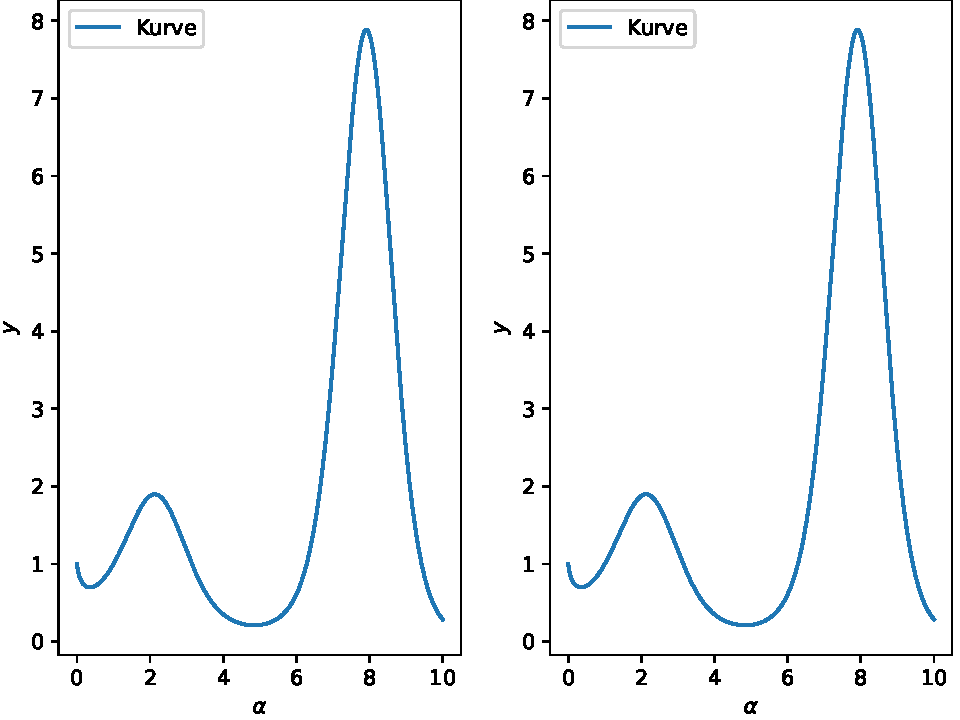
\includegraphics{plot.pdf}
  \caption{Zeitlicher Temperaturverlauf im wärmeren Reservoir.}
  \label{fig:plot}
\end{figure}


Siehe \autoref{fig:plot}!
